\chapter{Method}\label{ch:method}

This chapter presents a novel framework for addressing the dynamic clustering
problem. It begins with the introduction of a new class of transitions that
incorporates the recurrence of clusters over time, enabling a more realistic
modeling of evolving data streams. A new formulation of overlapping scores is
then proposed for both spherical and Gaussian clusters, allowing for an easy
thresholding for detecting overlapping between clusters. In addition, a
triggering mechanism based on the CluStream~\cite{clustream} micro-clustering
algorithm is introduced to detect significant structural changes in the data.
The chapter concludes with a detailed description of the framework's
architecture, outlining its components and their interactions in supporting
adaptive and interpretable streaming clustering.

\section{Extended Transitions}\label{sec:extended_transitions}

To more accurately capture the dynamic evolution of clusters over time, this
section introduces an extension to the traditional notion of transitions.
Instead of relying solely on pairwise comparisons or aggregate statistics,
transitions are modeled using a structured and interpretable representation. As
described in MEC~\cite{mec}, one effective approach is to represent transitions
between two clustering results as a \textbf{bipartite graph}. In this graph,
each node represents a cluster at a specific time point, and edges indicate the
presence of overlap between clusters across two consecutive timestamps.

This representation enables a methodical framework for identifying and
classifying transition patterns. Each edge encodes a correspondence between
clusters, allowing the system to categorize transitions such as
\emph{survivals}, \emph{splits}, \emph{merges}, \emph{appearances}, and
\emph{disappearances}, based on the edge connectivity patterns. The resulting
graph-based model facilitates a more expressive and insightful analysis of
cluster evolution.

\begin{figure}[H]
    \centering
    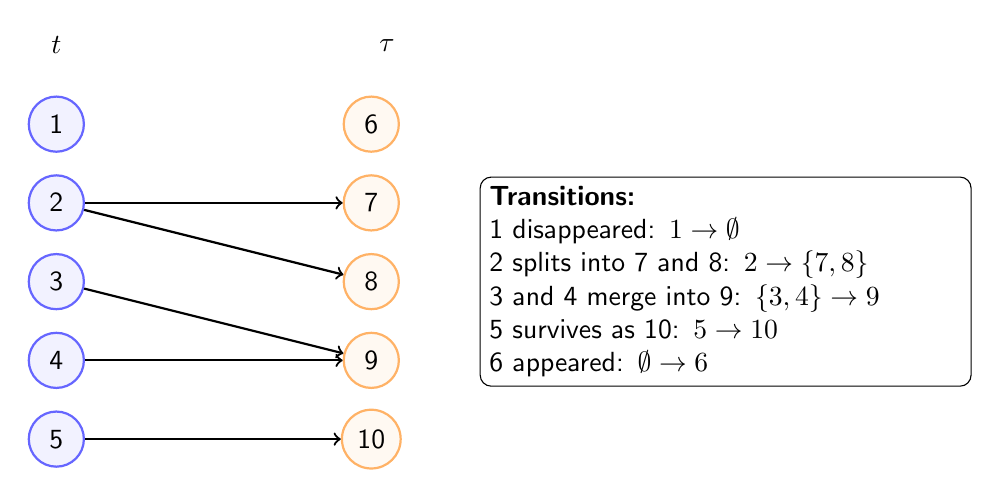
\begin{tikzpicture}[
            leftnode/.style={circle, draw=blue!60, fill=blue!5, thick, minimum size=7mm},
            rightnode/.style={circle, draw=orange!60, fill=orange!5, thick, minimum size=7mm},
            font=\sffamily,
            node distance=8mm and 30mm
        ]

        % Time labels
        \node[font=\bfseries] at (0,2) {$t$};
        \node[font=\bfseries] at (4.2,2) {$\tau$};

        % Left nodes (1 to 5)
        \node[leftnode] (n1) at (0,1) {1};
        \node[leftnode] (n2) at (0,0) {2};
        \node[leftnode] (n3) at (0,-1) {3};
        \node[leftnode] (n4) at (0,-2) {4};
        \node[leftnode] (n5) at (0,-3) {5};

        % Right nodes (6 to 10)
        \node[rightnode] (n6) at (4,1) {6};
        \node[rightnode] (n7) at (4,0) {7};
        \node[rightnode] (n8) at (4,-1) {8};
        \node[rightnode] (n9) at (4,-2) {9};
        \node[rightnode] (n10) at (4,-3) {10};

        % Edges
        \draw[->, thick] (n2) -- (n7);
        \draw[->, thick] (n2) -- (n8);
        \draw[->, thick] (n3) -- (n9);
        \draw[->, thick] (n4) -- (n9);
        \draw[->, thick] (n5) -- (n10);

        % Transitions legend centered vertically
        \node[align=left, anchor=center, text width=6cm, draw, rounded corners] (legend) at (8.5,-1) {
            \textbf{Transitions:} \\
            1 disappeared: $1 \rightarrow \emptyset$ \\
            2 splits into 7 and 8: $2 \rightarrow \{7, 8\}$ \\
            3 and 4 merge into 9: $\{3, 4\} \rightarrow 9$ \\
            5 survives as 10: $5 \rightarrow 10$ \\
            6 appeared: $\emptyset \rightarrow 6$
        };

    \end{tikzpicture}
    \caption{Example of transitions from clusters at time $t$ to clusters at time $\tau$.}
    \label{fig:cluster-transitions}
\end{figure}

To support fine-grained tracking and avoid ambiguity in complex transitions,
events such as merges and splits are decomposed into \textbf{atomic
      transitions}. Each atomic transition links a single source cluster to a
destination cluster (or vice versa), enabling a clearer interpretation of
compound transitions.

\begin{figure}[H]
    \centering
    \begin{minipage}{0.55\textwidth}
        \centering
        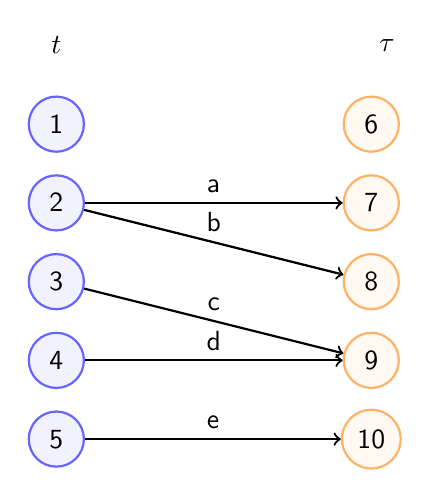
\begin{tikzpicture}[
                leftnode/.style={circle, draw=blue!60, fill=blue!5, thick, minimum size=7mm},
                rightnode/.style={circle, draw=orange!60, fill=orange!5, thick, minimum size=7mm},
                font=\sffamily,
                node distance=8mm and 30mm
            ]

            % Time labels
            \node[font=\bfseries] at (0,2) {$t$};
            \node[font=\bfseries] at (4.2,2) {$\tau$};

            % Left nodes (1 to 5)
            \node[leftnode] (n1) at (0,1) {1};
            \node[leftnode] (n2) at (0,0) {2};
            \node[leftnode] (n3) at (0,-1) {3};
            \node[leftnode] (n4) at (0,-2) {4};
            \node[leftnode] (n5) at (0,-3) {5};

            % Right nodes (6 to 10)
            \node[rightnode] (n6) at (4,1) {6};
            \node[rightnode] (n7) at (4,0) {7};
            \node[rightnode] (n8) at (4,-1) {8};
            \node[rightnode] (n9) at (4,-2) {9};
            \node[rightnode] (n10) at (4,-3) {10};

            % Edges
            \draw[->, thick] (n2) -- (n7) node[midway, above] {a};
            \draw[->, thick] (n2) -- (n8) node[midway, above] {b};
            \draw[->, thick] (n3) -- (n9) node[midway, above] {c};
            \draw[->, thick] (n4) -- (n9) node[midway, above] {d};
            \draw[->, thick] (n5) -- (n10) node[midway, above] {e};

        \end{tikzpicture}
    \end{minipage}
    \hfill
    \begin{minipage}{0.4\textwidth}
        \centering
        \begin{tabular}{|c|c|c|l|}
            \hline
            \textbf{Edge} & \textbf{From} & \textbf{To} & \textbf{Type} \\
            \hline
            -             & 1             & -           & Disappearance \\
            a             & 2             & 7           & Split         \\
            b             & 2             & 8           & Split         \\
            c             & 3             & 9           & Merge         \\
            d             & 4             & 9           & Merge         \\
            e             & 5             & 10          & Survival      \\
            -             & -             & 6           & Appearance    \\
            \hline
        \end{tabular}
    \end{minipage}
    \caption{Example of atomic cluster transitions between time $t$ and $\tau$.}
    \label{fig:atomic-cluster-transitions}
\end{figure}

The classification of transitions relies on analyzing the degree of
connectivity (i.e., number of incident edges) for each node in the bipartite
graph constructed between clustering results at times $t$ and $\tau$:

\begin{itemize}
      \item \textbf{At time $t$}:
            \begin{itemize}
                  \item A cluster with no outgoing edges is labeled as \emph{disappeared}.
                  \item A cluster with multiple outgoing edges is considered to have undergone a
                        \emph{split}.
            \end{itemize}

      \item \textbf{At time $\tau$}:
            \begin{itemize}
                  \item A cluster with no incoming edges is marked as \emph{newly appeared}.
                  \item A cluster with multiple incoming edges is the result of a \emph{merge}.
            \end{itemize}
\end{itemize}

When a cluster node at either time $t$ or $\tau$ has exactly one connecting
edge, the nature of the transition cannot be inferred directly from the graph
structure alone. In such cases, additional context is needed to disambiguate:

\begin{itemize}
      \item \textbf{From time $t$ to $\tau$}:
            \begin{itemize}
                  \item If the destination cluster has only one incoming edge, the transition is a
                        \emph{survival}.
                  \item If the destination cluster has multiple incoming edges, the source cluster has
                        \emph{merged} with others.
            \end{itemize}

      \item \textbf{From time $\tau$ to $t$}:
            \begin{itemize}
                  \item If the originating cluster has only one outgoing edge, the transition is a
                        \emph{survival}.
                  \item If the originating cluster has multiple outgoing edges, it has \emph{split}.
            \end{itemize}
\end{itemize}

When both nodes involved in a transition have exactly one edge but are each
involved in other connections, the transition is labeled as a
\textbf{mergesplit}, representing a complex reconfiguration that combines
merging and splitting behaviors.

\begin{figure}[H]
    \centering
    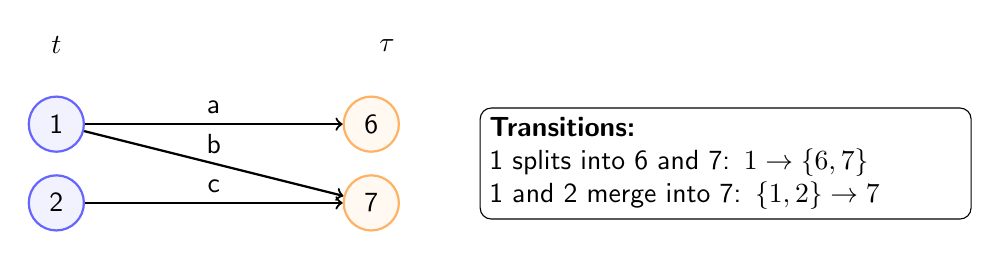
\begin{tikzpicture}[
            leftnode/.style={circle, draw=blue!60, fill=blue!5, thick, minimum size=7mm},
            rightnode/.style={circle, draw=orange!60, fill=orange!5, thick, minimum size=7mm},
            font=\sffamily,
            node distance=8mm and 30mm
        ]

        % Time labels
        \node[font=\bfseries] at (0,2) {$t$};
        \node[font=\bfseries] at (4.2,2) {$\tau$};

        % Left nodes
        \node[leftnode] (n1) at (0,1) {1};
        \node[leftnode] (n2) at (0,0) {2};

        % Right nodes
        \node[rightnode] (n6) at (4,1) {6};
        \node[rightnode] (n7) at (4,0) {7};

        % Edges
        \draw[->, thick] (n1) -- (n6) node[midway, above] {a};
        \draw[->, thick] (n1) -- (n7) node[midway, above] {b};
        \draw[->, thick] (n2) -- (n7) node[midway, above] {c};

        % Legend (left)
        \node[align=left, anchor=center, text width=6cm, draw, rounded corners] (legend) at (8.5,0.5) {
            \textbf{Transitions:} \\
            1 splits into 6 and 7: $1 \rightarrow \{6, 7\}$ \\
            1 and 2 merge into 7: $\{1, 2\} \rightarrow 7$
        };

    \end{tikzpicture}

    \vspace{1em}

    % Table below the diagram
    \begin{minipage}{0.8\textwidth}
        \centering
        \begin{tabular}{|c|c|c|l|}
            \hline
            \textbf{Edge} & \textbf{From} & \textbf{To} & \textbf{Transition Type} \\
            \hline
            a             & 1             & 6           & Split                    \\
            b             & 1             & 7           & Mergesplit               \\
            c             & 2             & 7           & Merge                    \\
            \hline
        \end{tabular}
    \end{minipage}
    \caption{Example of a mergesplit transition.}
    \label{fig:cluster-mergesplit}
\end{figure}

While the transitions discussed so far describe short-term structural changes
between consecutive timestamps, long-term dynamics often involve recurring
patterns. To support extended temporal analysis, three additional transition
types are introduced: \textbf{reappearance}, \textbf{remerge}, and
\textbf{resplit}.

\begin{itemize}
      \item \textbf{Reappearance} occurs when a cluster that previously
            disappeared re-emerges after a delay. To detect this, information
            about disappeared clusters is retained. If a new cluster in a future
            timestep significantly overlaps with one of these stored clusters, it
            is classified as a reappearance rather than a new appearance.

      \item \textbf{Remerge} describes a situation in which a previously
            merged cluster splits and, at a later point, its components reassemble
            into a similar structure. The system tracks the identities of the
            original components, allowing for recognition of this reformation.

      \item \textbf{Resplit} is the converse case, where clusters that
            previously resulted from a split later recombine. If the new merged
            cluster shows significant overlap with the original parent cluster,
            the event is identified as a resplit.
\end{itemize}

By incorporating these extended transition types, the framework enables not
only the detection of immediate structural changes but also the identification
of long-term recurrences. This allows for a more nuanced and temporally aware
analysis of cluster evolution in dynamic environments.

\section{Overlapping Scores Definition}\label{sec:overlapping_scores}
Overlapping scores are used to quantify the degree of similarity or interaction
between two clusters. In dynamic clustering, such scores play a crucial role in
understanding cluster evolution. This section introduces two novel
formulations: one tailored for spherical clusters, and one for Gaussian
clusters with arbitrary covariance structures.

\subsubsection*{Custom Overlapping Score for Spherical Clusters}

For clusters with approximately spherical shapes, the following \textbf{Custom
      Overlapping Score (CustomOS)} is proposed:

\begin{equation}\label{eq:custom_os}
      \text{CustomOS}(c_1, c_2) = 2^{- \frac{d(\mu_1, \mu_2)}{r_1 + r_2}}
\end{equation}

where:
\begin{itemize}
      \item $ d(\mu_1, \mu_2) $ is the Euclidean distance between the centers of clusters $ c_1 $ and $ c_2 $,
      \item $ r_1 $ and $ r_2 $ represent the respective radii of the clusters.
\end{itemize}

\textbf{Properties and Interpretation:}
\begin{itemize}
      \item The score is bounded in $ (0, 1] $, where:
            \begin{itemize}
                  \item $ \text{CustomOS} \to 0 $: the clusters are very distant.
                  \item $ \text{CustomOS} = 0.5 $: the clusters are tangent, i.e., $ d(\mu_1, \mu_2) = r_1 + r_2 $.
                  \item $ \text{CustomOS} = 1 $: the clusters are completely overlapped, i.e., $ d(\mu_1, \mu_2) = 0 $.
            \end{itemize}

      \item The score decays exponentially with the normalized inter-cluster distance,
            providing a \textit{scale-invariant} measure of similarity.

      \item The score can be interpreted as a \textbf{probability-like value} quantifying
            the likelihood that two clusters are evolutionarily related. The most uncertain
            case is when the clusters are tangent ($ \text{CustomOS} = 0.5 $), where:
            \begin{itemize}
                  \item $ c_2 $ could be the evolution of $ c_1 $ with a large center shift (i.e., $ d = r_1 + r_2 $),
                  \item or $ c_2 $ could represent a newly formed cluster that emerged near $ c_1 $.
            \end{itemize}

      \item Thanks to these properties, a natural threshold for deciding overlap is $
                  \epsilon = 0.5 $. Scores above this suggest potential continuity or evolution;
            scores below indicate separation.

      \item The score requires only the cluster centers and radii to compute, which makes
            it particularly suitable for \textbf{streaming clustering frameworks} where
            retaining all data points is infeasible. This supports lightweight and
            efficient computation.
\end{itemize}

\subsubsection*{Effective Overlapping Score for Gaussian Clusters}

Building upon the idea of the \textit{Custom Overlapping
      Score}~(\ref{eq:custom_os}), which assumes spherical symmetry, the
\textbf{Effective Overlapping Score (EffectiveOS)} generalizes the concept to
clusters modeled as multivariate Gaussian distributions. This allows for the
consideration of directional variability and correlated features by
incorporating covariance structure into the overlap estimation.

The \textbf{EffectiveOS} is defined as:

\begin{equation}
      \text{EffectiveOS} = 2^{\frac{-d_M(\mu_1, \mu_2)}{\text{RMSSize}_1 + \text{RMSSize}_2}}
\end{equation}

where $ d_M(\mu_1, \mu_2) $ is the Mahalanobis distance between the cluster
means:

\begin{align}
      d_M(\mu_1, \mu_2) & = \sqrt{(\mu_1 - \mu_2)^\top \Sigma_{12}^{-1} (\mu_1 - \mu_2)} \\
      \Sigma_{12}       & = \frac{\Sigma_1 + \Sigma_2}{2}
\end{align}

The term $ \text{RMSSize}_j $ represents the \textbf{root mean square size} of
cluster $ j $, capturing its generalized radius along principal directions:

\begin{align}
      \text{RMSSize}_j & = \sqrt{\frac{1}{n} \sum_{i=1}^n a_i^2} \\
      a_i              & = \chi^2_\alpha \sqrt{\lambda_i^j}
\end{align}

where:
\begin{itemize}
      \item $ \lambda_i^j $ are the eigenvalues of the covariance matrix $ \Sigma_j $,
            corresponding to the variance along each principal axis of cluster $ j $,
      \item $ \chi^2_\alpha $ is the critical value of the chi-squared distribution at
            confidence level $ \alpha $, scaling the eigenvalues to a desired confidence boundary.
\end{itemize}

\textbf{Properties and Intuition:}
\begin{itemize}
      \item \textbf{Generalization of Spherical Case:} When covariance matrices are multiples
            of the identity, the Mahalanobis distance reduces to the Euclidean distance, and
            RMSSize approximates the radius, thus reducing to the CustomOS formulation.
      \item \textbf{Covariance-aware Distance:} The Mahalanobis distance accounts for
            feature correlation and direction-dependent spread, making it suitable for ellipsoidal clusters.
      \item \textbf{Confidence-aware Scaling:} RMSSize uses the eigenvalue spectrum scaled
            by a chi-squared factor to describe the effective spatial extent of a Gaussian cluster
            with statistical rigor.
      \item \textbf{Probabilistic Interpretation:} Like CustomOS, the EffectiveOS is bounded
            in $ (0, 1] $ and can be interpreted as a probability-like measure of overlap or evolution
            likelihood.
      \item \textbf{Streaming-Friendly Implementation:} Although more complex than the CustomOS,
            the EffectiveOS still relies only on statistical summaries (means, covariances, and eigenvalues),
            making it applicable in streaming scenarios where raw data is discarded after summarization.
\end{itemize}

\section{Novel Triggering Strategy}\label{sec:novel_triggering_strategy}

\section{Proposed Framework}\label{sec:proposed_framework}

The architecture of the proposed dynamic clustering framework is illustrated in
Figure~\ref{fig:architecture}. It consists of multiple interconnected modules,
each dedicated to a specific aspect of processing and tracking clusters within
a data stream.

The streaming clustering component employs the CluStream
algorithm~\cite{clustream}, which supports distinct online and offline
clustering phases and allows the offline phase to be triggered on demand. Each
submodule—namely online, offline, and triggering—is also explicitly
represented.

The original algorithm's offline phase uses K-means with a fixed number of
clusters $ k $. In contrast, the offline phase is implemented using Gaussian
Mixture Models (GMMs)~\cite{gaussian_mixtures}, where the number of components
is determined based on the Silhouette metric. This approach helps relax the
spherical cluster assumption inherent in K-means and allows the number of
clusters to adapt to the underlying data distribution without requiring prior
knowledge of $ k $.

It is noted that in the original CluStream algorithm, the offline phase is
triggered based on a fixed time interval. As previously
stated,~\cite{namitha_dynamic_clustering_2} implements a mechanism that
triggers the offline phase using the Page-Hinkley algorithm to monitor the
distance between incoming data points and their closest microclusters.

In this work, a new triggering strategy specifically tailored to the CluStream
online phase is proposed. This strategy initiates the offline phase when the
number of significant changes in the online phase exceeds a predefined
threshold. A significant change is defined as either the deletion of an old
microcluster or the merging of existing microclusters, which occurs when a new
microcluster must be created to accommodate an incoming data point.

To better understand the workflow and responsibilities within the framework,
the following subsections describe the core modules and their roles:

\begin{itemize}

      \item \textbf{Online Phase (Microclustering):} The online module handles real-time
            summarization of the stream into microclusters. A microcluster is a compact
            structure that captures summary statistics (e.g., count, linear sum, and squared sum)
            of nearby data points in the feature space. This process compresses the incoming data
            into a manageable set of meaningful summaries while preserving essential distributional
            characteristics. It ensures that data is processed with low latency and prepares it
            for more complex downstream analysis.

      \item \textbf{Triggering Strategy:} Since performing macroclustering at every step
            would be inefficient, this module decides when to invoke the offline phase.
            It monitors the evolution of microclusters and can be based on fixed time intervals,
            statistical change detection. The triggering strategy ensures a balance between
            computational efficiency and responsiveness to changes in
            the data.

      \item \textbf{Offline Phase (Macroclustering):} When triggered, this module clusters the
            current set of microclusters to produce macroclusters—higher-level structures that
            summarize broader data trends. Algorithms such as K-Means or Gaussian Mixture
            Models may be applied to the weighted centers of microclusters. This step extracts
            interpretable patterns from the stream and forms the basis for cluster tracking.

      \item \textbf{History:} This module is specifically responsible for maintaining minimal
            yet sufficient information about past macroclusters in order to detect complex long-term
            transitions, namely \emph{reappearance}, \emph{remerge}, and \emph{resplit}.
            Instead of storing the full stream or detailed cluster content, it archives only
            essential descriptors (such as centroids, radii, and timestamps) of disappeared or
            transformed clusters. This historical memory allows the tracking module to compare
            newly formed clusters with previous ones and identify structural recurrences, enabling
            a deeper understanding of temporal cluster dynamics while ensuring low memory overhead.

      \item \textbf{Tracking:} The tracking module compares macroclusters across time to detect
            how clusters evolve. By computing overlap scores (e.g., CustomOS for spherical clusters
            or EffectiveOS for Gaussian ones) it identifies transitions.

\end{itemize}

\begin{figure}[H]
    \centering
    \begin{tikzpicture}[node distance=1.5cm and 2cm, every node/.style={font=\small}]
        % Nodes
        \node (stream) [diamond, draw, minimum height=0.1cm, minimum width=5cm, above, inner sep=0pt] {Streaming Data};

        \node (online) [rectangle, draw, rounded corners, text centered, minimum height=1cm, below=2cm of stream] {\shortstack{Online\\(Microclustering)}};

        \node (offline) [rectangle, draw, rounded corners, text centered, minimum height=1cm, below=of online] {\shortstack{Offline\\(Macroclustering)}};

        \node (trigger) [rectangle, draw, rounded corners, text centered, minimum height=1cm, right=of online] {Triggering Strategy};

        \node (tracking) [rectangle, draw, rounded corners, text centered, minimum height=1cm, below=of offline] {Tracking};

        \node (history) [ellipse, draw, text centered, minimum height=1cm, left=of tracking] {History};

        \node (report) [diamond, draw, text centered, minimum height=1cm, minimum width=4cm, below=2cm of tracking] {Report};

        % Arrows
        \draw[thick,->,>=stealth] (stream) -- (online);
        \draw[thick,->,>=stealth] (online) -- (offline);
        \draw[thick,->,>=stealth] (trigger) |- (offline);
        \draw[thick,->,>=stealth] (offline) -- (tracking);
        \draw[thick,->,>=stealth] (offline) -| (history);
        \draw[thick,->,>=stealth] (history) -- (tracking);
        \draw[thick,->,>=stealth] (tracking) -- (report);

        % Box
        \node[draw, dashed, inner sep=10pt, fit=(online)(offline)(trigger), label=above right:Streaming Clustering] {};
        \node[draw, dashed, inner sep=45pt, fit=(online)(offline)(trigger)(history)(tracking), label=below left:Dynamic Clustering] {};

    \end{tikzpicture}
    \caption{Proposed architecture for the dynamic clustering framework.}
    \label{fig:architecture}
\end{figure}


Together, these modules enable a flexible, efficient, and adaptive clustering
framework capable of capturing evolving patterns in streaming data while
maintaining interpretability and scalability.

The final \textbf{Report}, consolidates the output of the entire framework into
a comprehensive summary. It includes:
\begin{itemize}
      \item A table showing the status and properties of each macrocluster at every
            iteration.
      \item A table listing all detected transitions (e.g., splits, merges, survivals,
            reappearances).
      \item A graph-based visualization of transitions across all time points, extending
            the bipartite structure into a multi-step representation.
      \item A spatial visualization of the macrocluster evolution across iterations,
            showing changes in position and shape over time.
      \item A curated collection of representative data samples for each cluster at each
            timestamp.
      \item A series of quality plots evaluating the compactness and separation of
            macroclusters at every macroclustering step.
      \item A timeline plot that counts the number of updates performed in the online phase
            at the microcluster level, providing insight into streaming activity and drift.
\end{itemize}

This rich reporting structure not only aids in interpretation and debugging but
also enables users to analyze the evolution of data structures and validate the
clustering process both qualitatively and quantitatively.